\subsubsection{Klassebeskrivelser}
Herunder ses de forskellige modelklasser i \gls{SL} og der vil til hver klasse være en uddybende forklaring om dennes funktionalitet og ansvar\\

\textbf{Catalogue}\\
Denne klasse indeholder en liste af produktkategorier, der hver især selv indeholder en liste af produkter, se afsnit \ref{PRODUCTCATEGORY} om ProductCategory for yderligere info om disse. Catalogue er det katalog af produkter systemet indeholder og ved boot af et delsystem vil dette som regel kalde en GetCatalogueDetails kommando, som vil give dem en instans af Catalogue med alle produkter i deres enkelte produktkategorier i systemet.

\begin{figure}[H]
    \centering
    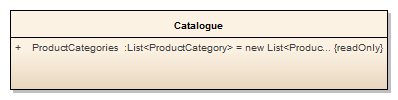
\includegraphics[width=0.6\textwidth]{Systemdesign/SharedLib/Images/Klasser/Model/Catalogue.png}
    \caption{Catalogue}
    \label{fig:klasseModelCata}
\end{figure}

\textbf{Product}\\
Denne klasse er meget brugt igennem hele systemet, den blev tidligt i udviklingen fastlagt så systemerne kunne udvides omkring dette koncept. Product indeholder alle data som for systemet er relevant omkring et produkt.

\begin{figure}[H]
    \centering
    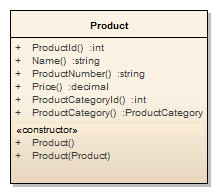
\includegraphics[width=0.4\textwidth]{Systemdesign/SharedLib/Images/Klasser/Model/Product.png}
    \caption{Product}
    \label{fig:klasseModelPrd}
\end{figure}


\textbf{ProductCategory}\label{PRODUCTCATEGORY}\\
Klassen ProductCategory kom ind i en senere iteration og gav muligheden for at placere produkter under samme kategori, f.eks. æble og pære under en kategori der hed "frugt".
ProductCategory har derfor som sagt et navn og derudover også en liste af produkter. 

\begin{figure}[H]
    \centering
    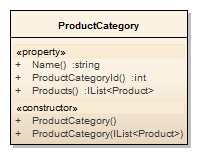
\includegraphics[width=0.4\textwidth]{Systemdesign/SharedLib/Images/Klasser/Model/ProductCategory.png}
    \caption{ProductCategory}
    \label{fig:klasseModelPrdCtg}
\end{figure}


\textbf{PurchasedProduct}\\
Klassen PurchasedProduct blev oprettet da der skulle implementeres funktionalitet omkring salg. Dette nødvendigjorde at der skulle et tidsstempel på produktet der var solgt og at der derudover skulle et antal (hvis flere af samme produkt var købt), prisen på daværende tidspunkt, da den nuværende pris på produktet godt kunne være ændret senere i databasen og til sidst en total pris, som bliver gjort op af antallet og stykprisen. Der blev derudover tilføjet et event til PurchasedProduct da denne også bliver brugt i \gls{KA}'s shoppinglist. Denne skulle vide hvornår antallet i en instans ændres, så grænsefladen kan ændre værdien på skærmen.

\begin{figure}[H]
    \centering
    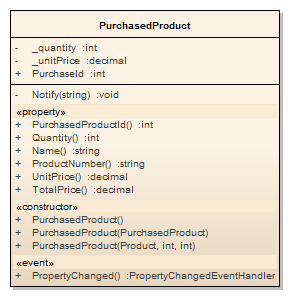
\includegraphics[width=0.6\textwidth]{Systemdesign/SharedLib/Images/Klasser/Model/PurchasedProduct.png}
    \caption{PurchasedProduct}
    \label{fig:klasseModelPurPrd}
\end{figure}


\textbf{Purchase}\\
Denne klasse sørger for at registrere køb fra \gls{KA}. Purchase klassen skal altså simulere et samlet køb af en eller flere varer og bliver derfor også brugt til at danne kvitteringer. Dette betyder altså at klassen har en liste af PurchasedProducts og et tidsstempel for købet.

\begin{figure}[H]
    \centering
    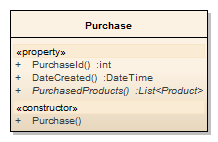
\includegraphics[width=0.4\textwidth]{Systemdesign/SharedLib/Images/Klasser/Model/Purchase.png}
    \caption{Purchase}
    \label{fig:klasseModelPurch}
\end{figure}



